\documentclass[xcolor=table]{beamer}
\usepackage[utf8]{inputenc}
\usepackage{default}
\usepackage{xspace,setspace}
\usepackage{amsmath,amsthm,amssymb}
\usepackage{ellipsis}
\usepackage[pdftex]{epsfig}
\usepackage{listliketab}
\usepackage[table]{xcolor}
\usepackage{booktabs}
\usepackage{amsmath}
\usepackage{amssymb}

\usepackage{pgf}
\usepackage{tikz}
\usetikzlibrary{arrows,automata}
\usetikzlibrary{graphs}
\tikzset{
     mainNode/.style =
        { circle
        , draw
        %, fill=blue!20,
        %, font=\sffamily\Large\bfseries
        }
}

\usetheme{AnnArbor}
%\usetheme{Berlin}
%\usetheme{Bergen}
%\usetheme{Antibes}
%\usetheme{Goettingen}
%\usetheme{Warsaw}
%\usetheme{Darmstadt}
%\usetheme{JuanLesPins}
%\setbeamertemplate{navigation symbols}{}
%\usecolortheme{beaver}
%\usecolortheme{rose}
%\usecolortheme{seagull}
%\usecolortheme{dove}
%\usecolortheme{seahorse}
%\usecolortheme{crane}
%\usepackage{color,colortbl}
%\usepackage{texnansi}
%\usepackage{marvosym}
%\usepackage{comment}


%\setbeamertemplate{frametitle}
%{\begin{centering}\smallskip
%   \insertframetitle\par
%   \smallskip\end{centering}}
%\setbeamertemplate{itemize item}{$\bullet$}
%\setbeamertemplate{navigation symbols}{}
%\setbeamertemplate{footline}[text line]{%
%    \hfill\strut{%
%        \scriptsize\sf\color{black!60}%
%        \quad\insertframenumber
%    }%
%    \hfill
%}

% Define some colors:

\definecolor{DarkFern}{HTML}{407428}
\definecolor{DarkCharcoal}{HTML}{4D4944}
\colorlet{Fern}{DarkFern!85!white}
\colorlet{Charcoal}{DarkCharcoal!85!white}
\colorlet{LightCharcoal}{Charcoal!50!white}
\colorlet{AlertColor}{orange!80!black}
\colorlet{DarkRed}{red!70!black}
\colorlet{DarkBlue}{olive!70!black}
\colorlet{DarkGreen}{green!70!black}
\definecolor{brickred}{RGB}{132,31,39}

% Use the colors:

%\setbeamercolor{title}{fg=Fern}
%\setbeamercolor{frametitle}{fg=Fern}
%\setbeamercolor{section title}{fg=Fern}
%\setbeamercolor{section in toc}{fg=Fern}
%\setbeamercolor{section name}{fg=Fern}
%\setbeamercolor{section in head/foot}{fg=Fern}
%\setbeamercolor{subsection title}{fg=Fern}
%\setbeamercolor{author}{fg=Fern}
%\setbeamercolor{normal text}{fg=Charcoal}
%\setbeamercolor{block title}{fg=black,bg=Fern!25!white}
%\setbeamercolor{block body}{fg=black,bg=Fern!25!white}
%\setbeamercolor{alerted text}{fg=AlertColor}
%\setbeamercolor{itemize item}{fg=Charcoal}

%\definecolor{bottomcolour}{rgb}{0.32,0.3,0.38}
%\definecolor{middlecolour}{rgb}{0.08,0.08,0.16}
\definecolor{tcsyellow}{RGB}{253,255,102}
\definecolor{tcsolive}{RGB}{77,147,191}
\definecolor{tcsolivemedium}{RGB}{147,177,210}
\definecolor{tcsolivelight}{RGB}{235,239,252}

\definecolor{skyolive}{rgb}{0.2,0.6,1}
\definecolor{darkolive}{rgb}{0.1,0.1,0.6}
\definecolor{darkred}{rgb}{1,0.2,0.1}
\definecolor{darkgreen}{rgb}{0.5,0.8,0.4}
\definecolor{Olive}{rgb}{0,0.3,0}
\definecolor{seagreen}{rgb}{0.3,0.9,0.6}
\definecolor{olive}{cmyk}{0.8,0.1,0.95,0.40}
\definecolor{golden}{cmyk}{0.0,0.25,0.85,0.15}
\definecolor{darkgolden}{cmyk}{0.0,0.27,0.94,0.07}
\definecolor{orange}{cmyk}{0.0,0.35,1.0,0.07}
\definecolor{orange2}{cmyk}{0.0,0.6,1.0, 0.0}
\definecolor{pecan}{cmyk}{0.0,0.37,0.80,0.12}
\definecolor{cadmium}{cmyk}{0.0,0.40,0.93,0.00}
\definecolor{snake}{cmyk}{0.8,0.1,0.95,0.60}
\definecolor{tcsyellow}{RGB}{253,255,102}
\definecolor{tcsolive}{RGB}{77,147,191}
\definecolor{tcsolivemedium}{RGB}{147,177,210}
\definecolor{tcsolivelight}{RGB}{235,239,252}

\definecolor{LRed}{rgb}{1,.8,.8}
\definecolor{MRed}{rgb}{1,.6,.6}
\definecolor{HRed}{rgb}{1,.2,.2}

\newtheorem{defn}{Definition}
\newtheorem{asf}{ASF Inputs}
\newtheorem{claim}{Claim}

\setbeamercolor{item projected}{bg=darkred}
\setbeamertemplate{enumerate items}[orange2]
\setbeamercolor{frametitle}{fg=white,bg=orange2}
\setbeamercolor{title}{fg=white,bg=orange2}
 
\usetheme{boxes}
\setbeamertemplate{blocks}[rounded][shadow=false]
\setbeamertemplate{itemize item}{\color{orange2}$\blacktriangleright$}
\setbeamertemplate{itemize subitem}{\color{orange2}$\blacktriangleright$}
 
\setbeamercolor{block title}{use=structure,fg=brickred,bg=white}
\setbeamercolor{block body}{use=structure,fg=black,bg=white}
 

\usefonttheme{professionalfonts}
% default | professionalfonts | serif |	structurebold | structureitalicserif |structuresmallcapsserif
%\usepackage{eulervm}

%% User defined commands
\newcommand{\vect}[1]{\ensuremath{\mathbf{#1}}}
\newcommand{\trans}[1]{\ensuremath{#1}^{\scriptsize{\textsf{T}}}}
\newcommand{\calX}{\ensuremath{{\cal X}}}
\newcommand{\calY}{\ensuremath{{\cal Y}}}
\DeclareMathOperator{\sign}{sign}
\DeclareMathOperator{\RSS}{RSS}
\DeclareMathOperator{\Var}{Var}

%\newtheorem{theorem}{Theorem}
\title{Linear Regression}
\begin{document}

\maketitle

\begin{frame}[t]
  \frametitle{Linear Regression}  
\begin{itemize}
    \item Simple approach to supervised learning when the target variable is 
        \textbf{continuous}.
    \item Assumes a linear relationship between the input variables 
        $x_1, \ldots, x_n$ and the target variable $y$.
    \item  When the target variable is discrete, the problem is a
    \textbf{classification}
        problem. 
  \end{itemize}
\end{frame}


\begin{frame}[t]
\frametitle{Linear Regression Models and Least Squares}
\begin{itemize}
    \item input vector $\trans{x} = (x_1, \ldots, x_n)$, output/response $y$
    \item linear model: $y = \theta_0 + \sum_{j=1}^{n} x_j \theta_j = \sum_{j = 0}^n
    x_j \theta_j$, where $x_0 = 1$
    \item $\theta$s are unknown parameters
    \item variables $x_j$ can come from different sources:
        \begin{itemize}
            \item quantitative inputs
            \item transformations of quantitative inputs: $\log$, $\sqrt{~}$ etc
            \item basis functions: $x_2 = x_1^2$, $x_3 = x_1^3$
            \item numeric encoding of the levels of qualitative inputs
            \item interactions between variables $x_3 = x_1 \cdot x_2$
        \end{itemize}
\end{itemize}
The model is \textbf{linear in the parameters $\theta$}.
\end{frame}

\begin{frame}[t]
\frametitle{Linear Regression Models and Least Squares~$\ldots$}
\begin{itemize}
    \item Typical situation: we have training data 
    \[(x^{(1)}, y^{(1)}), \ldots, (x^{(m)}, y^{(m)})\] 
    from which to estimate the parameters $\theta$.
    
    \item Least squares: pick parameters $\theta = \trans{(\theta_0, \ldots, \theta_n)}$ to minimize 
    \[J(\theta) = 
    \frac{1}{2} \sum_{i = 1}^{m} \left (y^{(i)} - \sum_{j = 0}^{n} x^{(i)}_j \theta_j \right )^2\]   
\end{itemize}

\pause

\begin{itemize}
    \item Gradient descent
    \item Analytical solution
    \item Probabilistic interpretation
\end{itemize}
\end{frame}

\begin{frame}[t]
\frametitle{Gradient Descent}
\begin{itemize}
    \item Start with an ``initial guess'' for $\theta$

    \pause

    \item Repeatedly perform the update for all $0 \leq j \leq n$:
    \[
        \theta_j := \theta_j - \alpha \frac{\partial}{\partial \theta_j} J(\theta),
    \]
    where $\alpha$ is the learning rate.

    \pause 

    \item For each $0 \leq j \leq n$:
    $
        \partial J(\theta)/ \partial \theta_j = - \sum_{i = 1}^m 
        \left ( y^{(i)} - \sum_{j = 0}^n x_j^{(i)} \theta_j \right ) \cdot x_j^{(i)}.
    $
    
    \pause

    \item Magnitude of update: a linear function of the input vectors, where the
    coefficients are the error terms $y - \sum_j x_j \theta_j$

    \pause

    \item Looks at every input in the training set before making an update: \pause
    \textbf{batch gradient descent}
    
    \pause

    \item Gradient descent is susceptible to \textbf{local minima} in general; in
    this case, $J$ is a \textbf{convex} function and has a \textbf{unique global
    minimum}.  
\end{itemize}
\end{frame}

\begin{frame}[t]
\frametitle{Stochastic Gradient Descent}
In batch gradient descent, the update step for the $j$th component is:
\[
    \theta_j := \theta_j  + \alpha \cdot \sum_{i = 1}^m 
        \left ( y^{(i)} - \sum_{j = 0}^n x_j^{(i)} \theta_j \right ) \cdot x_j^{(i)}.
\]

\begin{itemize}
    \item Has to scan through the entire training set for a \emph{single} update
    
    \item Costly operation if $m$ is large
    
    \pause

    \item \textbf{Stochastic Gradient Descent}: for every training instance $(x, y)$, 
    $x = \trans{(x_0, x_1, \ldots, x_n)}$, update the parameters:
    \[
         \theta_j := \theta_j  + \alpha \cdot \left ( y - \sum_{j = 0}^n x_j 
         \theta_j \right ) \cdot x_j.
    \]
\end{itemize}
\end{frame}

\begin{frame}[t]
\frametitle{Stochastic Gradient Descent: Features and Issues}
\begin{itemize}
    \item Doesn't have to look at the entire training set to make progress.

    \item Often gets close to the optimum much faster than batch gradient descent.

    \item May never converge to the optimum (can keep on oscillating between values 
    near the optimum). This problem is alleviated by choosing $\alpha$ to be very
    small.
\end{itemize}
\end{frame}

\begin{frame}[t]
\frametitle{Analytic Solution}
\[J(\theta) = 
    \frac{1}{2} \sum_{i = 1}^{m} \left (y^{(i)} - \sum_{j = 0}^{n} x^{(i)}_j \theta_j \right )^2\]  
Want to find in closed-form a value of $\theta$ that minimizes $J(\theta)$ 

\begin{itemize}
    \item Write $J(\theta)$ is matrix-vector form.
    
    \pause

    \item \textbf{Design matrix.} An $m \times (n + 1)$ matrix $X$ defined by:
    \[
        X = \left [ \begin{array}{ccc}
                        \hbox{---} & \trans{(x^{(1)})} & \hbox{---} \\
                        \hbox{---} & \trans{(x^{(2)})} & \hbox{---} \\
                        \vdots     & \vdots                   & \vdots     \\
                        \hbox{---} & \trans{(x^{(m)})} & \hbox{---} \\
                   \end{array}
            \right ]
    \]

    \pause

    \item $y = \trans{(y^{(1)}, \ldots, y^{(m)})}$
\end{itemize}
\end{frame}

\begin{frame}[t]
\frametitle{Analytic Solution $\ldots$}
\[y - X \cdot \theta =  \left [ \begin{array}{c} 
                                    y^{(1)} \\
                                    y^{(2)} \\
                                    \vdots \\
                                    y^{(m)}
                                \end{array}\right ] -
                        \left [ \begin{array}{c}
                                    \trans{(x^{(1)})} \cdot \theta \\
                                    \trans{(x^{(2)})} \cdot \theta \\
                                    \vdots                         \\
                                    \trans{(x^{(m)})} \cdot \theta \\
                                \end{array}
                       \right ]\]
Matrix-form of $J(\theta)$:
\begin{equation*}
\begin{split}
    J(\theta) & = \frac{1}{2} \sum_{i = 1}^{m} \left (y^{(i)} - \sum_{j = 0}^{n} 
                    x^{(i)}_j \theta_j \right )^2 \\
              & = \frac{1}{2} \trans{(y - X \theta)} (y - X \theta)
\end{split}
\end{equation*}
\end{frame}

\begin{frame}[t]
\frametitle{Analytic Solution $\ldots$}
Minimize $J(\theta)$ w.r.t $\theta$:
\begin{equation*}
\begin{split}
    \nabla_{\theta} J(\theta) & = \nabla_{\theta} \frac{1}{2} \trans{(y - X \theta)} (y - X \theta) \\
                              & = \text{see Andrew Ng's notes} \\
                              & = \trans{X} X \theta - \trans{X} y  
\end{split}
\end{equation*}
yielding: 
\[\boxed{\theta = (\trans{X} X)^{-1} \cdot \trans{X}y.}\] 

\pause

\begin{itemize}
    \item \textbf{Assumption:} $X$ has full column rank so that $\trans{X}X$ is invertible. \pause
    \emph{Proof.} Show that $\trans{X} X z = 0$ implies $z = 0$. 

    \pause

    \item If $X$ does not have full column rank, the usual strategy is to remove redundant columns.   
\end{itemize}
\end{frame}

\begin{frame}[t]
\frametitle{Probabilistic Interpretation}
\textbf{Assumptions}
\[
    y^{(i)} = \trans{\theta} \cdot x^{(i)} + \epsilon^{(i)},  
\]
where the error terms $\epsilon^{(i)}$
\begin{itemize}
    \item capture unmodeled effects and/or random noise

    \item are independent and identically distributed as $N(0, \sigma^2)$ 
\end{itemize}

\pause

\medskip

Given $x^{(i)}$, 
\begin{itemize}
    \item $E(y^{(i)} \mid x^{(i)}) = \trans{\theta} \cdot x^{(i)}$
    
    \pause

    \item $\Var(y^{(i)} \mid x^{(i)}) = \Var(\epsilon^{(i)}) = \sigma^{2}$
\end{itemize}

\pause

\medskip

Thus $y^{(i)} \mid x^{(i)} \thicksim N(\trans{\theta} x^{(i)}, \sigma^2)$:
\[
    p(y^{(i)} \mid x^{(i)} ; \theta ) = \frac{1}{\sqrt{2 \pi} \sigma} 
                        \exp{\left ( - \frac{(y^{(i)} - \trans{\theta} \cdot x^{(i)})^2}{2 \sigma^2}\right )}
\]
\end{frame}

\begin{frame}[t]
\frametitle{Maximum Likelihood Estimation}
\begin{itemize}
    \item Given $x = \trans{(x^{(1)}, \ldots, x^{(m)})}$ and $\theta$, what is the joint distribution of 
            the $y = \trans{(y^{(1)}, \ldots, y^{(m)})}$? 

    \pause
    
    \item Since the $\epsilon^{(i)}$s are independent: \pause 
        \[
            p(y \mid x ; \theta) = \prod_{i = 1}^{m} p(y^{(i)} \mid x^{(i)} ; \theta)
        \]

    \pause

    \item \textbf{Likelihood function.} $L(\theta) = p(y \mid x ; \theta)$ 

    \pause
        
    \[
        L(\theta) = \prod_{i = 1}^{m} \frac{1}{\sqrt{2 \pi} \sigma} 
            \exp{\left \{ - \frac{\left ( y^{(i)} - \trans{\theta} x^{(i)} \right ) ^2}{2 \sigma^2} \right \}}
    \]
    
    \pause

    \item \textbf{Principle of Maximum Likelihood.} Choose the parameters to make the data as likely 
        as possible. Choose $\theta$ to maximize $L(\theta)$.
\end{itemize}
\end{frame}

\begin{frame}[t]
\frametitle{Maximum Likelihood Estimation $\ldots$}
Maximizing $L(\theta)$ is equivalent to maximizing \emph{any} strictly increasing 
function of $L(\theta)$.

\pause

\begin{itemize}
    \item Usual to maximize the log likelihood $l(\theta) = \log L(\theta)$.

    \item $l(\theta) = m \log \frac{1}{\sqrt{2 \pi} \sigma} - 
                        \frac{1}{\sigma^2} \cdot \frac{1}{2} 
                            \sum_{i = 1}^{m}{\left ( y^{(i)} - \trans{\theta} x^{(i)} \right ) ^2}$.
    \item Maximizing $l(\theta)$ is equivalent to minimizing 
        $\frac{1}{2} \sum_{i = 1}^{m}{\left ( y^{(i)} - \trans{\theta} x^{(i)} \right ) ^2}$.
\end{itemize} 

\pause

\bigskip

\begin{block}{Summary}
Under the previous probabilistic assumptions: \textbf{least-squares regression} 
corresponds to finding the \textbf{maximum likelihood estimate} of $\theta$.
\end{block}
\end{frame}

\begin{frame}[t]
\frametitle{The Goodness of Fit}
\end{frame}

\begin{frame}[t]
\frametitle{Predicting House Prices}
\begin{center}
    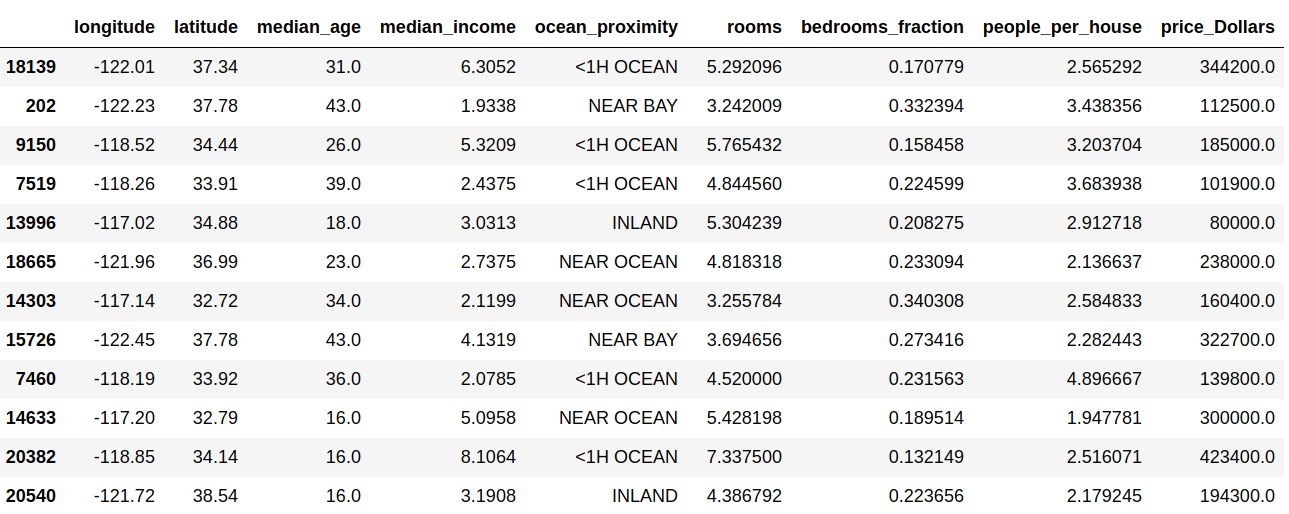
\includegraphics[scale=0.2]{housing_data.png}
\end{center}
\end{frame}

\end{document}
